\cchapter{کارهای مرتبط}
\label{related-works}

%%%%%%%%%%% معرفی Orchestration %%%%%%%%%%%%%%%%%%

قبل از بررسی درخت موضوعی بهتر است به مبجث ترکیب توابع در پلتفرم‌های بدون سرور بپردازیم. در \cite{bharti2021sequential} ۷ ترکیب  از توابع در FaaS بررسی شده است. البته این مقاله ذکر می‌کند که ۲ دسته‌بندی اصلی در رایانش بدون‌سرور داریم: \lr{MbaaS} و \lr{FaaS}. از \lr{MbaaS} به عنوان سرویس‌های سمت سرور برنامه‌های کاربردی وب و موبایل استفاده می‌کنند. پلتفرم Firebase یک نمونه از آن است. در حال حاضر این دسته‌از سرویس‌های ابری به شدت در حال توسعه است و البته، تمرکز این مقاله بر روی این موضوع هم نخواهد بود. 

یکی از چالش‌های اصلی معماری بدون سرور در ان است که برای تولید یک برنامه کاربردی بزرگ یا تجاری، باید جریان‌های کاری پیچیده‌ای را ایجاد کنیم. برای همین کار باید تعداد زیادی تابع را ایجاد کنیم که این توابع باید به اشکال مختلف هم‌دیگر را فراخوانی کنند. مثلا بعضا ممکن است یک تابع بعدی را فراخوانی کند یا یک تابع لازم باشد همزمان چند تابع را فراخوانی و اجرا کند و … . پیاده‌سازی یک راه حل درست برای این مورد بسیار برای رسیدن به معماری میکروسرویس برای ما مهم و حیاتی است و هرگونه کوتاهی و خطا در راه‌حل، باعث کارایی پایین محصول نهایی خواهد شد و با مشکلات بسیاری در پیاده‌سازی، ما را مواجه می‌سازد. 

برای حل این معضل، ارائه دهندگان خدمات تجاری اقدام به معرفی سرویس‌هایی تحت عنوان \lr{FaaS Orchestrator} نموده‌اند. هدف این سرویس‌ها ایجاد و پشتیبانی از ترکیب‌توابع و سناریو‌های پر‌کاربرد برای دستیابی به عملکرد روان در برنامه‌های کاربردی تحت پلتفرم بدون سرور است. دو پلتفرم معروف Orchestrator عبارتند از: \lr{AWS Step Functions} (با به اختصار \lr{ASF}) و دیگری \lr{IBM Cloud Function Sequences}.

توابع ترکیب شده توسط \lr{Orchestrator}ها حتما باید ۳ معیار را ارضا کنند: 

\begin{enumerate}
	
	\item ترکیبات توابع باید به‌ گونه‌ای باشند که جعبه سیاه بودن توابع نقض نشوند. یعنی فقط باید بتوانیم از روی ورودی و خروجی توابع محتوای آن را حدس زد.
	
	\item این ترکیب‌ها تابع قوانین و قواعد مشخصی باشند. همچنین، این ترکیبات باید قابل جایگزینی باشند.
	
	\item نباید بگونه‌ای فراخوانی اتفاق بیافتد که برای محاسبه‌ی هزینه همزمان پول ۲ تابع یا بیشتر را بدهیم\LTRfootnote{double billing}.
	
\end{enumerate} 

ما از این سه قانون با عنوان لم‌های بدون سرور\LTRfootnote{Serverless Trilemma} یاد می‌کنیم و هر ترکیبی از توابع که این ۳ معیار بالا را ارضا کند، \lr{ST-Safe} نامیده می‌شود. ترکیبات معروف توابع به شرح زیر است: 

\begin{enumerate}
	
	\item ترکیب با استفاده از بازتاب‌\LTRfootnote{Reflection}: به این صورت است که یک تابع اقدام فراخوانی سایر توابع به صورت همزمان \LTRfootnote{synchronous} می‌کند. در شکل \ref{fig:FaaS-Reflective-Pattern.png} یک نمونه مثال از فراخوانی همزمان توابع ذکر شده است. تنها مشکلی که دارد این است که با معضل \lr{Double billing} مواجه خواهیم شد. 
	
	\begin{figure}
		\centering
		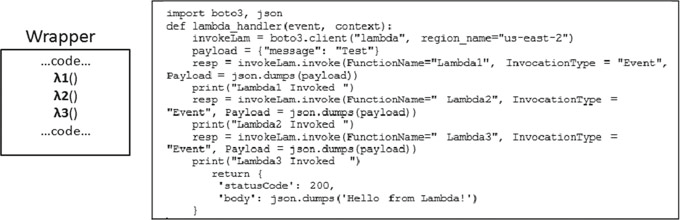
\includegraphics[width=\linewidth]{figs/FaaS-Reflective-Pattern.png}
		\caption {الگوی بازتابی در فراخوانی‌ها}
		\label{fig:FaaS-Reflective-Pattern.png}
	\end{figure}
	
	\item ترکیب همجوشی\LTRfootnote{Fusion} : در این حالت تابع \lr{wrapper}، توابعی که فراخوانی کرده‌ایم در تابع اصلی را بارگذاری می‌کند. مشکل اصلی آن این است که اصل جعبه سیاه را نقض می‌کند و همچنین باید توابع حتما با یک زبان نوشته شوند.  شکل \ref{fig:FaaS-Fusion-Pattern} یک الگوی همجوشی را نشان می‌دهد. 
	
	\begin{figure}
		\centering
		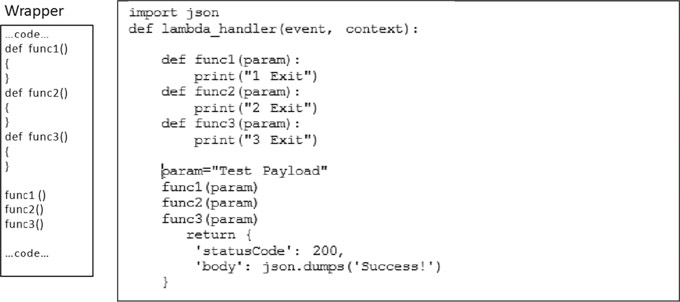
\includegraphics[width=\linewidth]{figs/FaaS-Fusion-Pattern}
		\caption {الگوی همجوشی در فراخوانی‌ها}
		\label{fig:FaaS-Fusion-Pattern}
	\end{figure}
	
	
	\item ترکیب غیرهمزمان: در این حالت،‌ تابع اول به فراخوانی تابع دوم می‌پردازد درحالی که اولی دیگر فعال نیست. این ترکیب نیز قانون دوم \lr{ST} را نقض می‌کند. 
	
	\item ترکیب توسط مشتری: در این حالت توابع ساخته می‌شود و خود مشتری خارج از سیستم بدون سرور اقدام به ترکیب توابع می‌کند. معروف ترین نمونه آن \lr{ASF} است و اصل اول را نقض می‌کند. 
	
	\item ترکیب زنجیره‌وار: در این ترکیب، یک ترکیب پس از اتمام اقدام به فراخوانی تابع بعدی می‌کند و همینطور ادامه پیدا می‌کند. این ترکیب مشکل \lr{double billing} دارد و \lr{ST-Safe} نیست. در شکل \ref{fig:FaaS-Chaining-Pattern} الگوی زنجیره‌ای نمایش داده‌شده است. 
	
	\begin{figure}
		\centering
		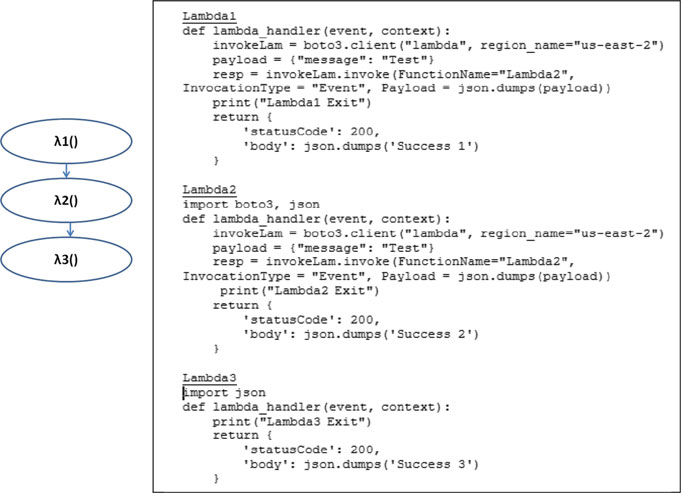
\includegraphics[width=\linewidth]{figs/FaaS-Chaining-Pattern}
		\caption {الگوی همجوشی در فراخوانی‌ها}
		\label{fig:FaaS-Chaining-Pattern}
	\end{figure}
	
\end{enumerate}

مقایسه‌ی این ترکیبات در جدول \ref{table:Function-Composition-Comparision} به طور خلاصه بیان شده است: \cite{baldini2017serverless}‌

\begin{table}
	\caption{مقایسه‌ی بین روش‌های ترکیب توابع}
	\begin{center}
		
		\begin{tabular}{| c | c | c | c |}
			\hline
			نوع ترکیب & پشتیبانی از \lr{poly glot} & کدام محدودیت ST نقض می‌شود؟ & مدت زمان اجرای برنامه تست \\
			\hline
			بازتاب & بله & پرداخت مجدد\LTRfootnote{Double Billing} & $311.0.$ \\
			\hline 
			همجوشی & خیر & جعبه‌سیاه\LTRfootnote{‌Black Box} & $2.47$ \\
			\hline
			غیرهمزمانی\LTRfootnote{Async} & نامشخص & نامشخص & نامشخص \\
			\hline
			ترکیب توسط مشتری\LTRfootnote{Client}  & بله & قاعده ترکیب توابع & $331.83$ \\
			\hline
			زنجیره‌ای & بله & پرداخت مجدد & $1104.78$ \\
			\hline
		\end{tabular}
		\label{table:Function-Composition-Comparision}
	\end{center}
\end{table}

در نهایت با مقایسه دو پلتفرم \lr{ASF} و \lr{IBM Cloud Function Sequences} برای یک برنامه تست مشابه به مدت‌زمان ‌های اجرای شکل \ref{FaaS-Orchestrators-Comparision-Runtim} می‌رسیم. 

\begin{figure}
	\centering
	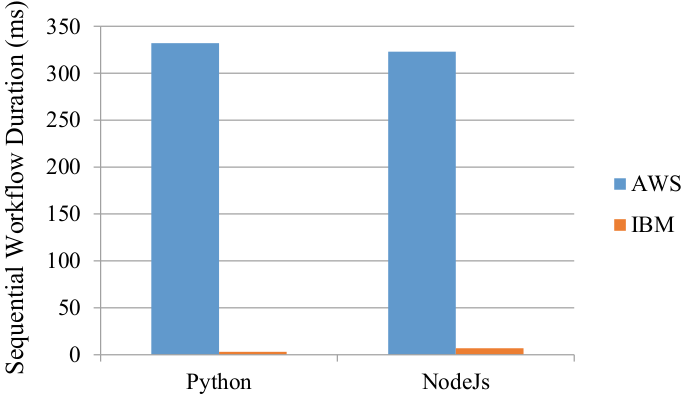
\includegraphics[width=\linewidth]{figs/FaaS-Orchestrators-Comparision-Runtime}
	\caption {مقایسه زمان اجرا ۲ برنامه مشابه با \lr{Node.js} و پایتون در دو پلتفرم \lr{ASF} و \lr{IBM Cloud Function Sequences}}
	\label{fig:FaaS-Orchestrators-Comparision-Runtime}
\end{figure}

%%%%%%%% درخت موضوعی %%%%%%%%%%%%%%%%%%%%%
\section{درخت موضوعی}

در این قسمت به بیان کارهای انجام شده در این حوزه خواهیم پرداخت و برای این کار درخت موضوعی مرتبط با آن رسم شده. هر گره ار درخت موضوعی یک راهکار برای جلوگیری از رخداد شروع سرد است و هر گره دارای بخش‌هایی است تا به برگ برسیم. در شکل \ref{fig:subject-tree} درخت موضوعی نمایش داده شده است و هر گره را به ترتیب بررسی خواهیم کرد. 

\begin{figure}
	\centering
	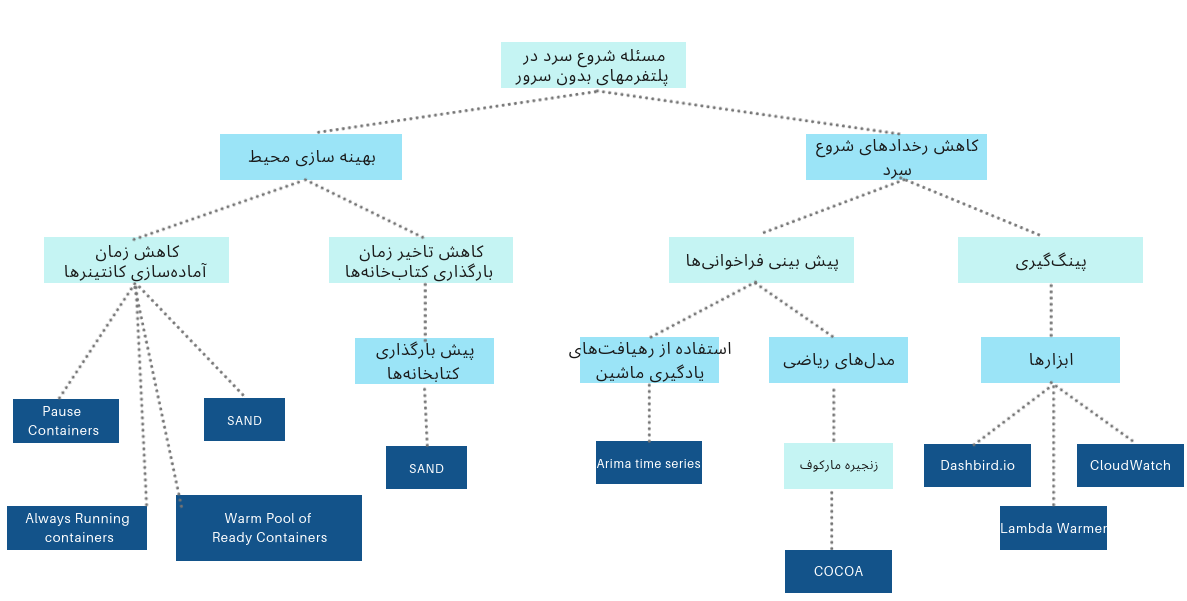
\includegraphics[width=\linewidth]{figs/subject-tree}
	\caption {درخت موضوعی}
	\label{fig:subject-tree}
\end{figure}

ریشه درخت مسئله شروع سرد است که ۲ گره اصلی دارد. گره سمت چپ که بهینه سازی محیط نام دارد، تلاش می‌کند تا در صورت وجود رخداد شروع سرد زمان آن‌را به حداقل برساند. این گره ۲ فرزند دارد که عبارتند از کاهش تاخیر آماده سازی کانتینرها و کاهش زمان بارگذاری کتابخانه‌ها. یک روش برای کاهش زمان بارگذاری کتاب‌خانه ها استفاده از روش پیش-بارگذاری است. 


گره سمت راست ریشه هم کاهش رخداد‌های شروع سرد است. تمرکز این گره در این است نگذاریم شروع سرد رخ دهد. گره سمت راست این نود، روش پینگ‌گیری است؛ در این روش سعی می‌کنیم با استفاده از ابزارهایی جلوگیری کنیم از سرد شدن توابع. در آخرین سطح این گره هم ابزارهای مرتبط معرفی شده‌اند. فرزند سمت چپ گره کاهش رخداد، پیش‌بینی فراخوانی‌ها است. در پیش‌بینی فراخوانی ها می‌توان از رهیافت‌های بدست آمده در یادگیری ماشین بهره جست. روش دیگر استفاده از مدل‌های ریاضیاتی غیریادگیری ماشین برای پیش‌بینی فراخوانی‌ها است. یکی از این روش‌های استفاده از ماشین‌ّهای حالت محدود بدست آمده با روش‌زنجیره مارکوف است.

 
در برگ‌های این درخت هرکدام یک مقاله را بررسی می‌کنیم. در ابتدا به توضیح درباره روش‌های بهینه‌سازی محیط می‌پردازیم و سپس به سراغ کاهش رخداد میرویم. در هر حوزه یک مقاله نمونه بررسی خواهد شد. 

\section{ بهینه سازی محیط}
          
          در این روش قرار به این است که مانع وقوع شروع سرد نشویم (در واقع هم نمی‌توان مانع از اتفاق شروع سرد شد)؛ بنابران به دنبال روش‌ یا روش‌هایی برای کاهش زمان شروع سرد هستیم. همانگونه که بالاتر ذکر کردیم، این موضوع را می‌توان از دو جنبه بررسی کرد. اول اینکه آماده‌سازی کانتینر‌ها را کاهش دهیم. روش دیگر این است که زمان لودشدن کتابخانه‌ها برای اجرای تابع را کاهش دهیم. برای این کار می‌شود از روش پیش-بارگذاری کتابخانه ها استفاده کرد.  
          
\subsection{کاهش زمان آماده‌سازی کانتینرها}

در این روش دنبال کمینه‌سازی زمان شروع سرد با استفاده از روش‌هایی برای کانفیگ بهینه محیط برای مواجهه با شروع سرد هستیم. عمده کارهایی که در این بخش انجام می‌دهیم در سطح شبکه یا کانتینر‌ها برای بهینه سازی است که روش‌های نسبتا سطح پایینی محسوب می‌شوند. 

یکی از مواردی که شروع سرد به شدت رخ می‌دهد، زمانی است که بنابه‌دلایلی تابع درخواست‌های زیادی دارد. این موضوع در \cite{lin2019mitigating} ذکر شده است. نویسنده معتقد با انجام این بهبودها در حدود 85٪ مدت‌زمان شروع سرد برای این توابع صرفه‌جویی خواهد شد. این مقاله از پلتفرم \lr{Knative} برای پیاده‌سازی تغییرات استفاده می‌کند. علت انتخاب \lr{Knative} این است که بر روی بستر کوبرنتیز ساخته می‌شود و از مفاهیمی مثل \lr{Pod} ها برای اجرای توابع و جریان‌های کاری استفاده می‌کند. بنابراین، از آنجایی که کوبرنتیز دست ما را برای انجام تغییرات باز می‌گذارد، می‌توان به آسانی به پیاده سازی سیاست‌های\LTRfootnote{policy} خودمان بپردازیم. در پلتفرم \lr{Knative} هر تابع در درون یک پاد اجرا می‌شود. پادها، ابتدایی‌ترین و ساده‌ترین بارهای‌کاری (به هر برنامه درحال اجرا در کوبرنتیز بارهای کاری می‌گوییم. توجه داشته باشید در کوبرنتیز بارکاری یک موجودیت نیست در واقع مفهومی است که به اجرای کانتینر‌ها و تخصیص \lr{CPU} و … اشاره دارد.) در کوبرنتیز هستند. در درون هر پاد تعدادی کانتینر اجرا می‌شود. در یک پاد شبکه‌ها، ذخیره سازی (Storage)‌ به صورت مشترک است. البته باز هم به خاطر وجود بحث‌هایی مثل \lr{Cgroups} و \lr{namespace} که ساختمان داده اصلی کانتینرها هستند، کانتینرهای داخل یک پاد از هم ایزوله هستند. پادهادر کوبرنتیز موجودیت‌های موقتی هستند و درصورت از دست رفتن نود، اتمام کار، کمبود منابع سرور و دلایل دیگر می‌توانند از سرور خارج شوند و دیگر قابل بازیابی نیستند. 

نکته‌ای که باید توجه داشت این است که یک پاد از جنس یک پردازه\LTRfootnote{Process} نیست؛ بلکه، محیطی منطقی برای اجرای کانتینر‌هاست و این کانتینرها هستند که از جنس پردازه‌ها هستند. داده‌های درون کانتینر‌ها وابسته به پادها هستند و با ری‌استارت شدن پادها محتویات ذخیره شده در کانتینرها از بین می‌روند مگر اینکه در ذخیره‌سازها ذخیره بشوند.\cite{KubernetesInAction}

با توجه به مقدماتی که در مورد پاد‌ها ذکر شد، اکنون منطقی به نظر می‌رسد برای مدیریت کانتینر‌ها بخواهیم از پادها استفاده کنیم و این رهیافت دست ما را برای اعمال تغییرات مختلف روی پلتفرم باز می‌کند. 

ما به صورت ایده‌آل دنبال کمترین سربار برای فراخوانی توابع هستیم. هنگامی که برای اولین بار تابع را فراخوانی می‌کنیم دچار تاخیر شروع سرد می‌شویم که در بخش ادبیات موضوع (رفرنس به شروع سرد)‌ در مورد آن مفصلا بحث کردیم. این مشکل در تمامی پلتفرم‌های بدون سرور، مشکل رایجی است. سربار شروع سرد را می‌توان به ۲ قسمت تعیین کرد :‌

\begin{enumerate}
	\item سربار ناشی از اجرای پلتفرم
	
علت اصلی این سربار اجرای پلتفرم است و به علت قرار گرفتن در صف یا دلایل دیگر باعث تاخیر می‌شود. از این دسته خطا‌ها می‌توان به network bootstraping، pod provisioning یا nework sidecar اشاره کرد. 
	
	\item سربار ناشی از خود اپلیکیشن
	
علت اصلی این سربار مشکلات خود برنامه است. این نوع تاخیر به مواردی از جمله زبان برنامه‌نویسی، حجم برنامه و نوع کتاب‌خانه‌هایی که از آن‌ها استفاده می‌کنیم بستگی دارد.
	
	
\end{enumerate}
 

برای مثال اجرای یک \lr{HTTP Server} ساده شروع سردی در حدود 5 ثانیه را به خود اختصاص می‌دهد؛ درحالی‌که با اجرای یک برنامه کلاس‌بندی عکس زمان شروع سرد به چیزی در حدود 40 ثانیه هم برسد. 

بنابراین، ایده این مقاله این است که برای اجرای توابعی که اخیرا محبوب شد‌ه‌اند از رهیافت استفاده از یک استخر گرم برای نگه‌داری این پاد استفاده‌کنیم. دقت کنید که در اینجا، در داخل هر پاد تنها یک کانتینر که آن کانتینر هم برای یک تابع است، اجرا می‌شود. هرگاه که درخواست جدید برای تابع می‌رسد در ابتدا استخر گرم را چک می‌کنیم که آیا پاد در آن موجود است یا خیر؟ اگر پاد در آن وجود داشت دیگر منتظر نمی‌مانیم، سریع تابع را در پلتفرم اجرا کرده و دیگر تاخیر شروع سرد را نخواهیم داشت. بنا به محاسبه نویسنده مقاله، این روش تا 85٪ زمان شروع سرد را برای توابع \lr{on-demand} نسبت به حالت عادی، کاهش می‌دهد. 

اما چگونه این تغییرات انجام شده است؟ شکل \ref{fig:knative-architecturea} نمایشگر معماری پلتفرم بدون سرور \lr{Knative} است. انتظار داریم با بهینه‌سازی‌هایی این رهیافت را برای مدیریت شروع‌های سرد اعمال کنیم. 

\begin{figure}
	\centering
	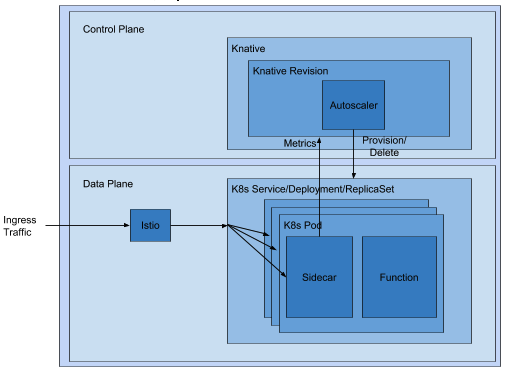
\includegraphics[width=\linewidth]{figs/knative-architecture}
	\caption {معماری پلتفرم Knative}
	\label{fig:knative-architecture}
\end{figure}

همانگونه که در این شکل می‌بینیم، وظیفه مولفه \lr{autoscaler}،  انجام وظایف مربوط به \lr{Scale up/down} است. هنگامی که دچار شروع سرد می‌شویم، مولفه \lr{autoscaler} دستور به ساخت پاد را می‌دهد  ولی از آنجایی که این امر وقت گیر است انجام آن بسیار طول می‌کشد. نهایتا اینکه پس از مدت زیادی پاد ساخته شده و داخل بخش \lr{data plane} اجرا می‌شود.

برای حل این مشکل، مقاله پیشنهاد می‌دهد تا در بخش \lr{control plane} و داخل \lr{revision} پلتفرم \lr{knative} یک مولفه مدیریت استخر قرار دهیم که آن با توجه به درخواست‌هایی که برای \lr{auto-scaler} می‌رسد، اقدام به ساخت پاد‌هایی و نگه‌داری آن در استخر گرم که در بخش \lr{data plane} توسعه داده شده، می‌کند. استخر گرم محدودیت ‌هایی مثل اندازه استخر دارد و تنها تعداد محدودی پاد در آن می‌توان نگه داشت.  حال اگر درخواستی برای پلتفرم برسد، \lr{autoscaler} ابتدا از کنترل کننده استخر\LTRfootnote{pool controller} وضعیت موجودی در استخر گرم را بررسی می‌کند. اگر در استخر پاد موجود باشد در اینصورت بلافاصله مهاجرت(migration)  از استخر گرم به سرویس رخ می‌دهد. از آنجایی که در استخر گرم منابع به پاد اختصاص داده شده و پاد کاملا آماده‌ی اجرا است؛ بنابراین، تاخیر شروع سرد بسیار ناچیزی خواهیم داشت. اما از طرفی، اگر پاد در استخر گرم موجود نباشد، دچار تاخیر شروع سرد خواهیم شد. نکته‌ی منفی این روش این است که در صورت رخداد شروع سرد، به میزان تاخیر‌های قبل، تاخیر ناشی از استعلام از استخر گرم ‌هم اضافه خواهد شد. شکل \ref{fig:Knative-architecture-modified} مدل جدید مقاله برای مدیریت شروع سرد را نشان می‌دهد. \cite{KubernetesInAction} 

\begin{figure}
	\centering
	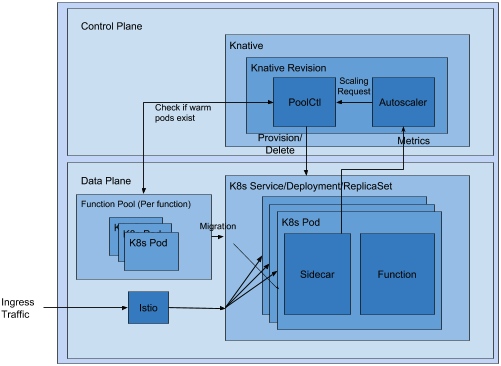
\includegraphics[width=\linewidth]{figs/Knative-architecture-modified}
	\caption {معماری پیشنهادی مقاله برای حل تاخیر شروع سرد}
	\label{fig:Knative-architecture-modified}
\end{figure}

\par
\par
مقاله دیگری که در این حوزه اقدام به بررسی تاثیر آماده سازی کانتیرها پرداخته از ایده pause container ها که مفهومی در کوبرنتیز است استفاده می‌کند. \ref{mohan2019agile}
این مقاله اقدام به بررسی تاخیر شروع سرد ناشی از اجرای همزمان تعدادی تابع کرد و نتایج خروجی آن را در شکل \ref{fig:coldstart-importance} نشان داده‌اند. 

در این واقع، این مقاله تاخیر شروع سرد را ناشی از آماده سازی کانتینر‌ها می‌بیند و سعی می‌کند تا حد امکان با آن مقابله کند. برای نمایش و پیاده‌سازی سناریو خود از پلتفرم‌ \lr{Apache OpenWhisk} استفاده کرده‌اند. طبق همان شکل نتیجه می‌گیریم که بخش عمده‌ای از تاخیرها ناشی از تاخیر در آماده‌سازی کانتینرها است، زیرا باید گام‌های طولانی برای ساخت و استقرار یک کانتینر و اختصاص شبکه به آن برداریم. شکل \ref{fig:container-network-creation} این گام ها را نشان می‌دهد.

\begin{figure}
	\centering
	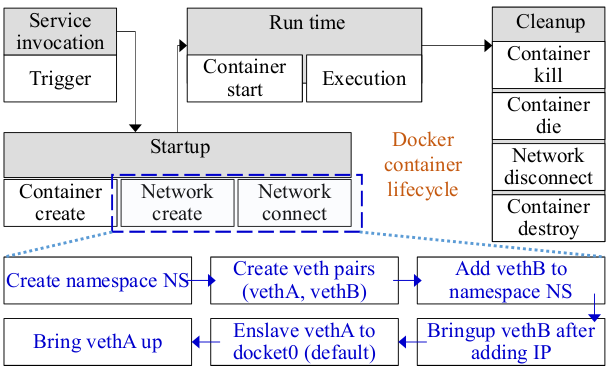
\includegraphics[width=\linewidth]{figs/container-network-creation}
	\caption {مراحل ساخت یک فضای نام در داکر}
	\label{fig:container-network-creation}
\end{figure}

همانگونه که در شکل مشخص است برای اجرای یک تابع در پلتفرم، ابتدا باید کانتیر آن ساخته شود. بسیاری از پلتفرم‌ها از جمله پلتفرم \lr{OpenWhisk} - که این مقاله تغییرات را بر بستر این پلتفرم بدون سرور انجام می‌دهد، - ازموتور داکر به عنوان موتنو کانتینری در پلتفرم خود پشتیبانی می‌کنند. در این موتور مراحل شکل فوق باید انجام بشود تا یک کانتینر کاملا آماده شود.

با توجه به شکل، تمامی بهبودهایی که باید انجام دهیم در مرحله شروع اولیه کانتینر است، جایی که دقیقا 3 مرحله داریم. ساخت کانتینرها، ساخت شبکه‌ها و اتصال کانتینرها به آن‌ها و در نهایت اتصال شبکه‌ها. 

در مرحله‌ای اول باید فضای نام‌را برای هر شبکه ایجاد کنیم. این کار در داکر توسط یک ویژگی کرنل لینوکس به نام فضای نام \LTRfootnote{namespace} انجام می‌گیرد. فضای نام یه مانع یا ایزوله کننده شبکه است که فرایند مختلف را از یکدیگر جدا می‌کند. در هر فضای نام پس از ایزوله سازی می‌توان مطمئن بود که دسترسی به پردازه‌های دیگر به شدت محدود شده است. اما، ما به دنبال ایزوله کردن پروسه نیستیم، بلکه به دنبال این هستیم که اجرا پردازه در سیستم عامل ایزوله باشد ولی ارتباط با آن نیز ممکن باشد. بنابراین باید تنظیمات شبکه در آن را انجام دهیم. 

بنابراین به دنبال ایجاد جفت‌های \lr{veth} \LTRfootnote{namespace} هستیم. جفت‌های \lr{veth} یک سری کابل مجازی هستند ( به طور دقیق از جنس خط لوله‌ها در سیستم عامل هستند) که وظیفه انتقال یک طرفه از کانتینر به فضای بیرون از آن و بالعکس را دارا می‌باشند. پس اقدام به اضافه کردن \lr{veth}ها به شبکه می‌کنیم. این دوقسمتی که مطرح شد خود شامل 6 مرحله کلی می‌شود که توضیح آن در این گزارش جایی ندارد.

حال نقش شبکه‌ها در شروع سرد چیست؟‌ همانگونه که قبلا گفتیم، هر کانتینر از 4 مرحله می‌گذرد. مرحله اول، مرحله فراخوانی سرویس هاست که در آن یک درخواست ساخت کانتینر برای \lr{docker daemon} ارسال می‌شود. مرحله دوم مرحله آغاز‌کردن\LTRfootnote{Startup} نام دارد که در طی آن یک کانتینر باید برای اتصال به محیط پیرامون آماده شود بنابراین کانتینر ساخته شده، شبکه درون و بیرون کانتینر کانفیگ می‌شود و به هم متصل می‌شوند.. مرحله سوم مرحله اجرا\LTRfootnote{execution} است که در طی آن، تابع اجرا می‌شود و در انتها مرحله‌ی نهایی یا مرحله پاکسازی\LTRfootnote{Cleanup} را داریم که شامل توقف اجرای کانتینر، قطع اتصال شبکه و نابود سازی آن است. \cite{DockerInAction}

علاوه ساخت کانتینرها،‌ به این توجه کنید که ما به دنبال اجرای همزمان آن‌ها نیز هستیم. این مورد زمان و سربار اجرا را نیز به طرز قابل توجهی بالا می‌برد.	اگر به شکل \ref{fig:coldstart-importance} نگاه کنید مجددا می‌بینید که به ازای اجرا‌های همزمان، زمان آماده‌سازی بسیار طولانی‌تر شده است درحالی‌که، زمان اجرا تغییر چندانی نکرده است. 

مقاله می‌گوید که بر طبق آمارهای گرفته شده، در مرحله آماده‌سازی کانتینرها، 90٪ زمان آماده‌سازی مربوط به ۲ مرحله ساخت شبکه‌ها و اتصال شبکه‌ها می‌شود. بنابراین معتقد است که با بهبود در این وضعیت تاخیر شروع سرد تا حد قابل توجهی برای تمامی توابع، کاهش خواهد یافت. حال مشکل اینجا‌است که این مراحل به کندی انجام می‌شوند مثلا برای ساخت شبکه این کار یکی یکی و در یک صف به نوبت انجام می‌شود. با توجه به اینکه در پلتفرم‌های بزرگ و تجاری در هر لحظه تعداد زیادی کانتینر باید ساخته یا حذف شوند این تاخیر به شدت افزایش پیدا خواهد کرد. برای اینکار آزمایشی انجام شد که نتایج آن در جدول \ref{table:1} قابل مشاهده است. 
\par

\begin{table}[h]
	\begin{center}
		\caption{زمان ساخت و پاکسازی کانتیرهای همزمان}
		\begin{tabular} {| c | c | c | c | c |}
			\hline
			
			تعداد فضا‌های نام همزمان & $1$ & $10$ & $50$ & $100$ \\
			\hline
			زمان ساخت & $0.28$ & $1.27$ & $6.28$ & $14.41$ \\
			\hline
			زمان پاکسازی & $0.20$ & $0.71$ & $3.24$ & $7.77$ \\
			\hline
		\end{tabular}
	\label{table:1}
	\end{center}
\end{table}

همانگونه که در این جدول قابل مشاهده است، زمان آماده‌سازی سرویس‌ها به ازای تعداد تعداد کانتینرهای همزمان، به طور نمایی افزایش می‌یابد. در حالی‌که ما در پلتفرم‌های تجاری همزمان تعداد زیادی کانتینر را هم بسازیم یا از بین ببریم. 

بهتر است به این دید نگاه کنیم که \lr{pause container} ها از قبل شبکه را ساخته و کانفیگ‌های مربوطه را انجام داده‌اند. پس کانتینری که در درون آن اجرا می‌شود تنها به معرفی برای اختصاص آدرس IP دارند که کار زمان‌بری نیست. بنابراین، می‌توان پس از ساخت یک کانتینر، تنها به اجرای آن در \lr{pause container} ها بپردازیم و از این طریق در زمان ساخت بسیار صرفه جویی کنیم. همچنین برای پاکسازی تنها باید کانتینر تابع مربوطه را حذف کنیم و \lr{pause container} بازیابی می‌شود. این رهیافت در شکل \ref{fig:pause-container-solution} نشان داده شده است.

\begin{figure}
	\centering
	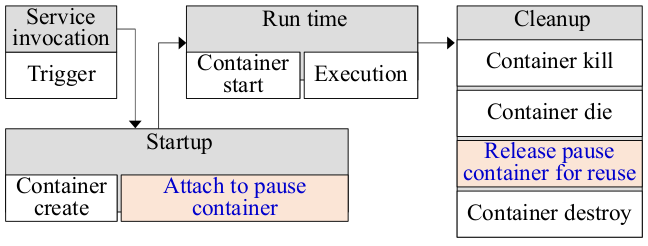
\includegraphics[width=0.8\linewidth]{figs/pause-container-solution}
	\caption {استفاده از \lr{Pause Container}ها برای کاهش تاخیر شروع سرد}
	\label{fig:pause-container-solution}
\end{figure}

در این حالت دو مرحله ساخت و اتصال شبکه جایگزین شده. همچنین برای مدیریت \lr{pause container} ها نیز یک استخر مربوط به آن‌ها ساخته‌شده است. در شکل \ref{fig:Pause-Container-Pool-Manager} نحوه عملکرد این رهیافت توضیح داده شده است.

\begin{figure}
	\centering
	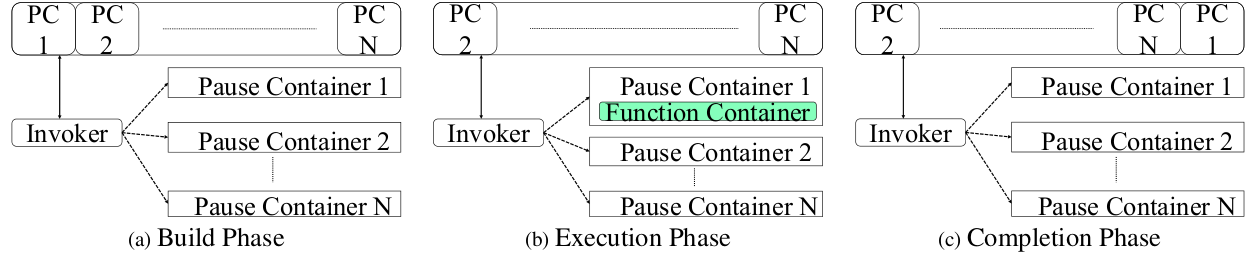
\includegraphics[width=\linewidth]{figs/Pause-Container-Pool-Manager}
	\caption {مدیر استخر \lr{Pause Container}ها}
	\label{fig:Pause-Container-Pool-Manager}
\end{figure}
 
در قسمت اول که فاز ساخت است۷ از قبل تعدادی کانتینر ساخته شده و در یک صف نگهداری می‌شوند. یک فراخواننده\LTRfootnote{invoker} داریم که وضعیت تمامی PC\LTRfootnote{مخفف Pause Container}ها را می‌داند. در قسمت بعدی می‌خواهیم یک تابع را اجرا کنیم؛ برای اینکار تنها کافی‌است که آن کانتینر را درون PC بارگذاری کنیم. و هرگاه کار تابع تمام شد تنها کافی است آن کانتینر در \lr{PC} را نابود کنیم. در انتها خود \lr{PC} بازیابی می‌شود و به انتهای صف استخرهای \lr{PC} اضافه می‌شود. 

نتایج این رهیافت در شکل زیر نشان داده شده است و می‌تواند تا 80٪ زمان شروع سرد را برای توابع کاهش دهد. برای مقایسه میزان بهبود داده شده شکل را با شکل مقایسه کنید.


\begin{figure}
	\centering
	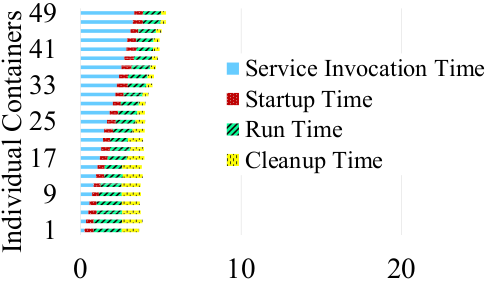
\includegraphics[width=0.8\linewidth]{figs/Pause-Containers-Results}
	\caption {نتیاج و بهبود حاصل شده با استفاده از \lr{Pause Container}ها}
	\label{fig:Pause-Containers-Results}
\end{figure}

%%%%%%%%%%%%%%%%%%%%%%% کاهش رخداد‌های شروع سرد%%%%%%%%%%%%%%%%%%%%%%%%%%%%%%%%%%%%

\section{کاهش رخداد‌های شروع سرد}

در این قسمت به دنبال روش‌هایی برای کاهش احتمال شروع سرد در پلتفرم‌های بدون سرور هستیم. در واقع ما به دنبال این هستیم که جلوی رخداد شروع سرد را با هایی بگیریم. از دسته‌بندی‌های کلی در این مبحث می‌وان به روش‌های جلوگیری از شروع سرد با استفاده از پینگ‌گیری یا روش‌های پیش‌بینی شروع سرد، اشاره کرد. روش دیگر برای جلوگیری از اتفاق شروع سرد عبارت‌است از پیش‌بینی شروع سرد. در این مرحله با استفاده از مدل‌های ریاضی و روش‌های یادگیری ماشین می‌توانیم شروه سرد را پیش‌بینی کنیم. توضیحات مربوط به هرکدام در زیر‌بخش مربوطه آمده است. 

	%%%%%%%%%%%	پینگ گیری %%%%%%%%%%%%%%%%%%%%%%%%%%

\subsection{پینگ‌گیری}

در این روش‌ها ما به دنبال کاهش تعدادی شروع‌های سرد در چرخه فراخوانی‌های یک تابع در پلتفرم، با استفاده از ابزارهایی برای جلوگیری از سرد شدن آن تابع هستیم. شیوه عملکرد این ابزارها به این‌گونه است که اقدام به فراخوانی توابع در بازه‌های زمانی مشخص برای جلوگیری از سرد شدن تابع می‌شوند. اگرچه ممکن است این روش ها کارایی خوبی از نظر مصرف منابع نداشته باشند، اما به دلیل ارزانی و سادگی استفاده و همچنین تطابق با پلتفرم‌های حال حاضر، محبوبیت قابل توجهی دارند. بنابراین، با استفاده از ابزارهای آماده‌ای مثل \lr{cloudwatch}\cite{CloudWatch} که برای مانیتور کردن سیستم توسعه داده شده یا افزونه‌هایی مثل \lr{Lambda Warmer}\cite{LambdaWarmer} که روی پلتفرم \lr{AWS Lamba} نصب می‌شود به سادگی شروع‌های سرد را کاهش داد. اتفاقا این روش با توجه به پشتیبانی خوب از پلفترم‌ها و سادگی استفاده در صنعت با اقبال بیشتری نسبت به روش‌های ابتکاری دیگر مواجه شده است. روش‌های ابتکاری بیشتر در حوزه پژوهش برای ایجاد روشی که بعدا در صنعت استفاده شود، هستند. درحالی‌که، عمده مقالات این قسمت در پیاده‌سازی و استفاده‌های صنعتی با این تکنیک است. در ادامه توضیحات بیشتری خواهیم داد. 
\subsubsection{استفاده از ابزار‌ها}

همانگونه که گفتیم، ابزار‌ها نقش جدی در مقابله با شروع سرد در صنعت برای برنامه‌های پیاده‌سازی شده در صنعت را دارند. در مقاله \cite{lloyd2018improving} همین موضوع به خوبی بیان شده. برای اینکار مقاله به دنبال پیاده سازی یک برنامه‌ با معماری monolithic برروی پلتفرم بدون سرور هستیم. بنابرین لازم است از کل اپلیکیشن به عنوان یک میکروسرویس استفاده کنیم و اقدام به راه‌اندازی برنامه کنیم. این موضوع علی‌رغم سربار زیاد و عدم رعایت استاندارد‌های بهترین تمرین\LTRfootnote{Best Practice}، در عمل قابل انجام است. بنابراین این کار را می‌کنیم. برنامه‌ای که در ابتدا کانتینرایز و سپس مستقر می‌شود یک برنامه‌کاربردی برای محاسبات حجم روان‌آب‌های ناشی از بارش‌های باران در حوزه محصولات محیط زیستی است. این برنامه به این صورت است که یک سری خروجی می‌گیرد و جدول روان آب‌ها در مناطق مختلف آمریکا را محاسبه می‌کند. 

مشکلی که با این برنامه‌داریم این است که باید حداقل زمان پاسخ را برای حداقل 100 درخواست همزمان داشته باشد. بنابراین لازم است از روش‌هایی مانع سرد شدن این سیستم شد. همچنین در هر لحظه باید حداقل 100 کانیتنر گرم‌هم برای رسیدگی به درخواست‌ها داشته باشد. برای این‌کار باید پس از استقرار نرم‌افزار یک اسکریپت برای فراخوانی 100 کانتینر به صورت همزمان داشته باشیم. این گونه می‌توان 100 بار کاری همزمان داشت.

حال باید از چرخه ذوب/یخ زدن\LTRfootnote{freeze/thaw} جلوگیری کرد تا بارهای کاری ما همیشه زنده باشند. برای این‌کار می‌توان اسکریپتی نوشت که هر چند‌وقت یکبار اقدام به فراخوانی 100 تابع همزمان کند. برای اینکار باید خود سروری که این برنامه‌را اجرا می‌کند همیشه زنده باشد و این یک چالش است اگر تنها بخواهیم از پلتفرم‌های FaaS برای اجرای آن اسکریپت استفاده کنیم. 

راه حل بعدی استفاده از ابزار‌های یا افزونه‌های\LTRfootnote{extensions} مربوطه برای جلوگیری از سرد شدن است. در این مقاله البته از ابزار \lr{Cloud watch} برای این منظور استفاده شده است. در این مقاله هر 5 دقیقه نسبت به پینگ‌گیری از توابع برای جلوگیری از سرد شدن اقدام کرده اند. 

از جمله نتیجه‌گیری های مقاله همچنین پایین رفتن کارایی پلتفرم بدون سرور در حین اجرای تعداد توابع همزمان است که در شکل \ref{fig:Serverless-AveragePerformace-PerNumberOfFunctions} نشان داده شده است. 

\begin{figure}
	\centering
	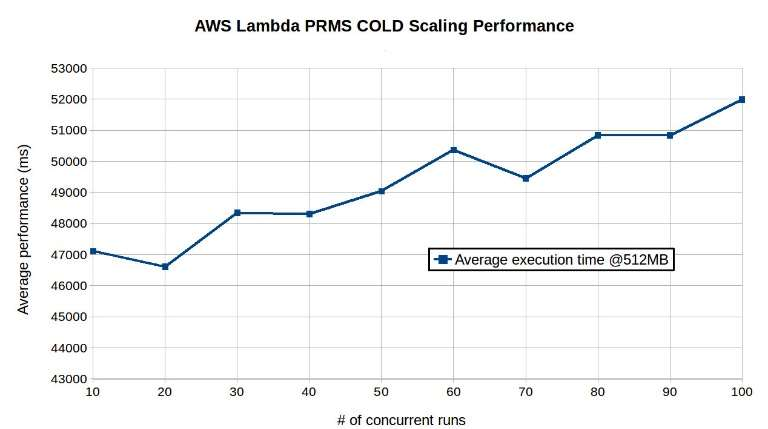
\includegraphics[width=0.8\linewidth]{figs/Serverless-AveragePerformace-PerNumberOfFunctions}
	\caption {متوسط کارایی (زمان اجرا)، به تعداد کانتنر‌های درحال اجرا}
	\label{fig:Serverless-AveragePerformace-PerNumberOfFunctions}
\end{figure}

تصویر \ref{fig:Serverless-AveragePerformace-PerNumberOfFunctions} یکی از مواردی است که حتما باید به آن توجه داشته باشیم. چون باید محاسبه کنیم به ازای تعداد کانتینر‌های در حال اجرا باید انتظار چه میزان متوسط زمان پاسخ را داشته باشیم. این خود یکی از موارد مهم در مقایسه با سایر روش‌های اجرای پروژه است. 

حال نویسنده این رهیافت را با روش استفاده از \lr{VM} ها از نظر اقتصادی و زمان اجرا مقایسه کرده است که نتیجه‌ی آن جدول \ref{table:Cost-Keepalive-Comparision}  است. 


\begin{table}
	\begin{center}
		\caption{مقایسه هزینه در به ازای استفاده از سیستم بدون سرور با بازه‌های فراخوانی \lr{Keep-Alive} مختلف در مقایسه با ماشین‌های مجازی}
		
		\begin{tabular}{| c| c | c |}
			\hline
			نوع زیرساخت & هزینه کلی در سال & صرفه‌جویی \\
			\hline
			\lr{Lambda + EC2} با بازه‌های زمانی 3  دقیقه برای KeepAlive & $\$4496.76$ & $892\%$ \\
			\hline
			\lr{Lambda + EC2} با بازه‌های زمانی 4  دقیقه برای KeepAlive & $\$4487.71$ & $893\%$ \\
			\hline
			\lr{Lambda + EC2} با بازه‌های زمانی 5  دقیقه برای KeepAlive & $\$4484.00$ & $894\%$ \\
			\hline
			\lr{Lambda + CloudWatch} با بازه‌های زمانی 5  دقیقه برای KeepAlive & $\$2278.06$ & $1759\%$ \\
			\hline
			\lr{Lambda + CloudWatch} با بازه‌های زمانی 4  دقیقه برای KeepAlive & $\$2847.57$ & $1407\%$ \\
			\hline
			سرویس \lr{Spot EC2} & $\$12579.84$ & $319\%$ \\
			\hline 
			سرویس \lr{On-demand EC2} & $\$40077.00$ & مبنای پایه \\
			\hline
		\end{tabular}
		\label{table:Cost-Keepalive-Comparision}
	\end{center}
\end{table}

\subsection{پیش‌بینی فراخوانی‌ها}

در این دسته‌بندی، قرار است مضرات استفاده از سیستم پینگ‌گیری را به حداقل برسانیم. در سیستم پینگ‌گیری با استفاده از فراخوانی در بازه‌های مشخص مانع از اتفاق افتادن شروع سرد می‌شویم ولی از طرفی بازدهی کمی داریم. یعنی اصلا از مزیت ویژگی ‌\lr{Scale-to-zero} که از ویژگی‌های کلیدی در پلتفرم‌های بدون سرور است استفاده‌ای نکرده ایم. برای پیش‌بینی شروع سرد می‌توانیم از روش‌های ریاضی یا از یادگیری ماشین برای پیش‌بینی شروع سرد استفاده کنیم. 

%%%%%%%%%%%%%%%%%%%%%%%%%%%%%%%استفاده از مدل‌های ریاضی %%%%%%%%%%%%%%%%%%%%%%%%%%
\subsubsection{استفاده از مدل‌های ریاضی }

متن تست

%%%%%%%%%%%%%%%%%%%%%% استفاده از روشهای یادگیری ماشین %%%%%%%%%%%%%%%%%%%
\subsubsection{استفاده از رهیافت‌های یادگیری ماشین}

روش دیگر برای پیش‌بینی شروع سرد، استفاده‌ از رهیافت‌های مبتنی بر یادگیری ماشین است. این موضوع در مقاله x مورد بررسی واقع شده است. البته این مقاله تنها به کاربرد استفاده از روش‌های یادگیری ماشین برای جلوگیری از اتفاق افتادن شروع سرد بسنده نمی‌کند بلکه رویکرد اصلی این مقاله – یا بهتر است بگوییم این دسته از مقاله‌ها -، استفاده از روش‌های یادگیری ماشین در کنار سایر روش‌ها برای این موضوع است. در مقاله \cite{shahrad2020serverless} از مدل \lr{Arima} در کنار روش‌های دیگر به عنوان یک روش مکمل استفاده شده است تا به بازدهی بهتری برای مدیریت شروع‌های سرد برسیم. 

ابتدای مقاله‌، تقسیم بندی‌هایی برای فعالساز‌های توابع\LTRfootnote{Triggers} داریم. توابع به 7 دسته اصلی تقسیم می‌شوند که عبارتند از: 

\begin{enumerate}
	\item \lr{HTTP}
	\item درخواست‌های صف\LTRfootnote{Queue}
	\item رخداد\LTRfootnote{Event}
	\item درخواست‌های \lr{Orchestration}
	\item زمانبند\LTRfootnote{Timer}
	\item حافظه\RTLfootnote{درخواست‌هایی مثل ارتباط با پایگاه داده در ذیل آن قرار می‌گیرد.}
	\item سایر درخواست‌ها
\end{enumerate}

در شکل \ref{fig:Azure-Trigger-invocations} نسبت تعداد توابع و نسبت فراخوانی‌ها در پلتفرم \lr{Azure} آمده است:‌

\begin{figure}
	\centering
	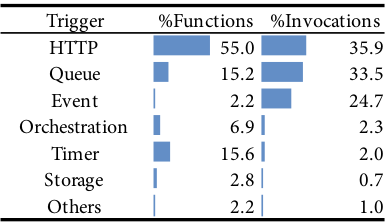
\includegraphics[width=0.8\linewidth]{figs/Azure-Trigger-invocations}
	\caption {تعداد و میزان فراخوانی فعال‌سازها در پلتفرم \lr{Azure}}
	\label{fig:Azure-Trigger-invocations}
\end{figure}

پرسشی که مطرح می‌شود این است که آیا برنامه‌ها تنها از یک نوع فعال‌ساز استفاده می‌کنند؟ جواب منطقا خیر است. برنامه‌های کاربری قاعدتا از انواع ترکیبات ممکن است استفاده کنند. مثلا می‌دانیم یک برنامه‌کاربردی ساده تحت وب حتما از ترکیب حافظه\LTRfootnote{Storage} و فراخوانی‌های HTTP حتما استفاده می‌کند. بنابراین نمی‌توان چنداد تفکیک قائل شد. درصد ترکیبات فعال‌ساز‌ها در شکل \ref{fig:Azure-function-compositions-applications} نشان داده شده است. 

\begin{figure}
	\centering
	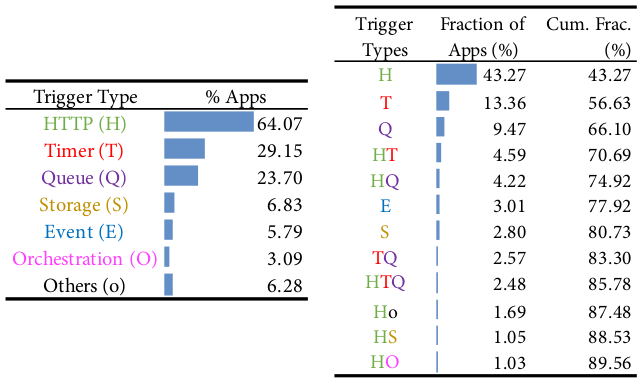
\includegraphics[width=0.7\linewidth]{figs/Azure-function-compositions-applications}
	\caption {نسبت ترکیب فعال‌سازها در برنامه‌های کاربردی}
	\label{fig:Azure-function-compositions-applications}
\end{figure}

آمارهایی برای درصد استفاده از توابع داریم که برای درک اهمیت شروع سرد مفید است. مثلا در 75٪ از توابع، زمان اجرای برنامه زیر 10 ثانیه است. بنابراین شروع سرد وقوع شروع سرد زمان اجرا را ممکن است تا 200٪ هم بالا ببرد. حدود ۸۱٪ توابع حداکثر 1 فراخوانی در دقیقه را ثبت می‌کنند یعنی اینکه زمان زنده‌ماندن\LTRfootnote{Keep-Alive} بالا برای این توابع اصلا به صرفه نیست. نکته جالب این است که کمتر از 20٪ توابع مسئول فراخوانی 99.6٪ از توابع هستند. 

مقاله به دنبال یک سیاست‌گذاری خودتطبیق برای سازگاری با شرایط است که برحسب آن زمان زنده بودن تابع تفاوت کند. برای تنظیم سیاست خودتطبیق از فلوچارت شکل \ref{Azure-‌Hybrid-Policy-flowchart} برای سیاست‌گذاری پیروی می‌کند. 


\begin{figure}
	\centering
	\includegraphics[width=0.8\linewidth]{figs/Azure-‌Hybrid-Policy-flowchart}
	\caption {تنظیم سیاست‌گذاری}
	\label{fig:Azure-‌Hybrid-Policy-flowchart}
\end{figure}

بر اساس شکل \ref{fig:Azure-‌Hybrid-Policy-flowchart} سه سیاست اصلی برای مواجهه با شروع سرد داریم

\begin{enumerate}
	\item برنامه خطای خارج از محدودیت\LTRfootnote{Out of Bound} نمی‌دهد.
	
	\begin{enumerate}
		\item الگوی برنامه قابل شناسایی است.
		
		در این حالت از روش هیستوگرام استفاده می‌کنیم. در این حالت دو متغیر زمانی \lr{Pre-Warm} و \lr{Keep-Alive} را تعریف می‌کنیم. وظیفه متغیر Prewarm این است که بلافاصله پس از اجرای تابع آن را به مدت زمانی مقرر شده سرد کند. این متغیر برای توابعی کاربرد دارد که الگوی فراخوانی آن‌ها به گونه‌ای است که تابع پس از فراخوانی تا مدتی را بلا استفاده می‌ماند. کاربرد متغیر Keep-Alive هم در این است که تابع پس از اتمام Pre-warm که مجددا گرم می‌شود تا چه زمانی گرم بماند. 
		
		ترکیب این دو در تصویر \ref{fig:Azure-Prewarm-keepalive-composition} به خوبی نشان داده شده است. 
		
		\begin{figure}
			\centering
			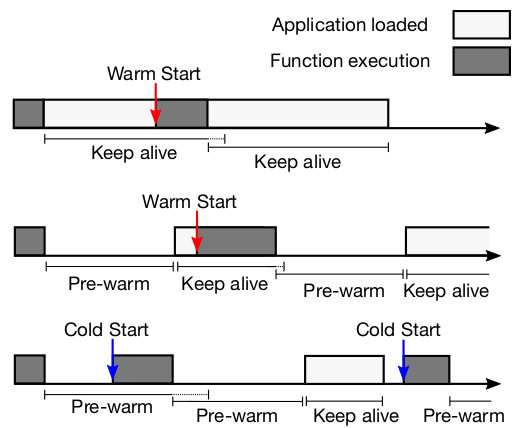
\includegraphics[width=0.7\linewidth]{figs/Azure-Prewarm-keepalive-composition}
			\caption {ترکیب Pre-Warm و keep-alive برای پیاده سازی شروع سرد برای الگوی شناسایی شده}
			\label{fig:Azure-Prewarm-keepalive-composition}
		\end{figure}
		
		نکته ای که باید به آن توجه داشت این است که Pre-warm را برای صرفه‌جویی در مصرف منابع پیاده سازی کرده‌ایم و  حتی ممکن است باعث شروع‌سردهای بیشتری هم بشود. 
		
		\item الگوی برنامه قابل شناسایی نیست.
		
		در این حالت از روش \lr{fixed-alive-time} استفاده می‌شود که همان روش سنتی برای مقابله با شروع سرد است. 
		
	\end{enumerate}
		
	\item برنامه خطای خارج از محدودیت می‌دهد.
	
	در این روش از روش پیش‌بینی فراخوانی براساس مدل ARIMA استفاده می‌شود. توضیحات نحوه عملکرد این مدل در \cite{ARIMA} ذکر شده است. 
\end{enumerate}

نتیجه استفاده از این روش در شکل \ref{fig:Azure-Hybrid-Arima-Usage-Result} آمده است. 

\begin{figure}
	\centering
	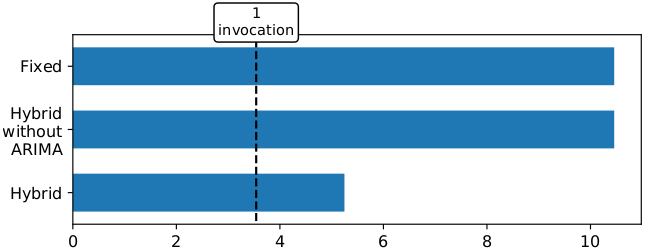
\includegraphics[width=0.7\linewidth]{figs/Azure-Hybrid-Arima-Usage-Result}
	\caption {مقایسه استفاده از 3 سیاست‌گذاری  مقابله با شروع سرد}
	\label{fig:Azure-Hybrid-Arima-Usage-Result}
\end{figure}

همانگونه که در شکل \ref{fig:Azure-Hybrid-Arima-Usage-Result} می‌بینیم، استفاده از روش هیبریدی درصد شروع‌های سرد را به زیر 6٪ رسانده است در حالی‌که در این آمار اولین شروع سرد که در حدود 3.8٪ از شروع‌های سرد را محاسبه می‌کند آمده است. در حالی که در دو سیاست دیگر میزان اتفاق افتادن شروع‌های سرد بالای 10٪ است پس از این نظر سیاست‌گذاری هیبریدی برای مدیریت شروع‌های سرد بسیار موثر است. 